\section{Experimental Evaluation}
\label{sec:results}

We evaluate \Treebeard{} on several machines. The first machine has an AMD Ryzen 9 7950X 16-Core processor,
128 GB of RAM, an NVIDIA RTX 4060 GPU with 8 GB of RAM and runs Ubuntu 22.04.2 LTS with CUDA 11.5. The 
second has an Intel Core i9-11900K (Rocket Lake) processor with 8 physical cores, 128 GB of RAM, an 
NVIDIA T400 with 2GB of RAM and runs Ubuntu 20.04.3 LTS with CUDA 11.8. We also evaluate \Treebeard{} on 
an AMD MI210 GPU. To establish the efficacy of \Treebeard{}, we compare it with NVIDIA RAPIDs v23.10,
Tahoe, and XGBoost v1.7.6. We use the same benchmark models as in the \TreebeardOLD{} paper\cite{Treebeard}.
We also evaluate \Treebeard{} on a set of randomly generated models.

\subsection{Performance on Random Models}
\begin{itemize}
  \item Generated a set of over 700 random models with varying depths (6, 7, 8), number of trees (100 - 1000 in steps of 100), 
  and number of features (powers of 2 between 8 to 1024 inclusive).
  \item Compared the kernel time speedup of \Treebeard{} vs RAPIDs on the RTX 4060. The schedule used was the one picked by the auto-tuner. 
  \item Speedups range between 1.5$\times$ and 8$\times$. \Treebeard{} outperforms RAPIDs on all models and batch sizes tested.
  \item Figure \ref{fig:randomModels4060} shows the speedup for models of depth 8 and batch size 512 and depth 6 and batch size 4096.
  Trends for other batch sizes and depths are similar.
\end{itemize}

\begin{figure*}[ht]
  \centering
  \begin{subfigure}[b]{.45\textwidth}
    \subcaptionbox*{}{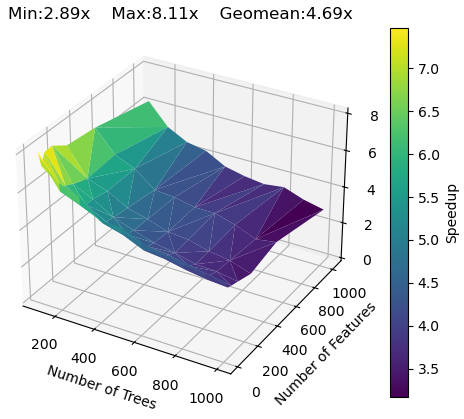
\includegraphics[width=\textwidth]{figures/RandomModels/kernel_speedup_b512_depth8.png}}
    \caption{Batch size 512, depth 8}
  \end{subfigure}
  \begin{subfigure}[b]{.45\textwidth}
    \subcaptionbox*{}{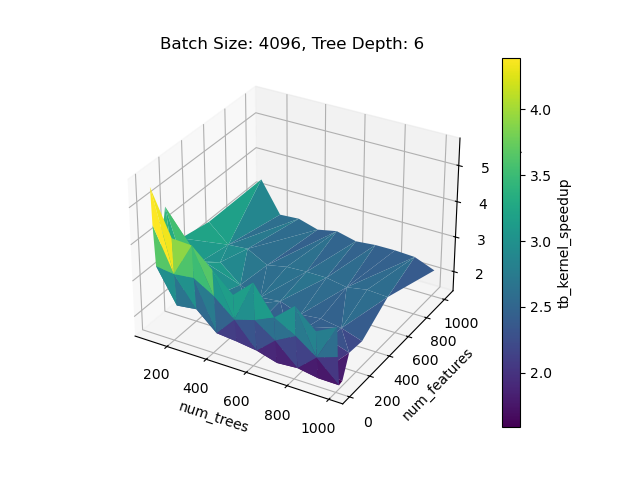
\includegraphics[width=\textwidth]{figures/RandomModels/kernel_speedup_b4096_depth6.png}}
    \caption{Batch size 4096, depth 6}
  \end{subfigure}
  \hfill
  \caption{\label{fig:randomModels4060}\Treebeard{} vs RAPIDs Kernel Time Speedup on NVIDIA RTX 4060 for several randomly generated models.}
\end{figure*}

\subsection{Comparison with RAPIDs, Tahoe and XGBoost}
\begin{itemize}
  \item Measured both the kernel time and total time (time including transferring data to the 
  GPU and results back) for RAPIDs and \Treebeard{}.
  \item Tahoe only allows us to measure the kernel time since it is written as an executable 
  that performs inference repeatedly on the same data that is transferred to the GPU once.
  \item Tahoe does not support multiclass models. We just ran the multiclass models (\op{covtype} and \op{letters})
  as regression models for the comparison. Tahoe also gives wrong results (as reported by its own tests) for 
  \op{letters} and \op{year}. In these cases, we pick the time of the fastest variant that gives the correct results.
  \item Compared the kernel time and total time speedup of \Treebeard{} vs RAPIDs on the RTX 4060 and T400.
  \item Compared the total time speedup of \Treebeard{} vs XGBoost on the RTX 4060.
  \item The schedule used was the one picked by the auto-tuner.
  \item \Treebeard{} outperforms RAPIDs at all batch sizes as shown in Figure \ref{Fig:TBvsRAPIDsTahoe_4060_Speedup}. 
  \item \Treebeard{} outperforms Tahoe on all models and batch sizes tested. Individual benchmark speedups range between 1.1$\times$ and 16$\times$.
  \item \Treebeard{} is faster than XGBoost by more than an order of magnitude. Results are not shown because the speedups don't fit on the same graph.
  \item Figure \ref{Fig:TBvsRAPIDs_4060_TotalTimeSpeedup} shows that \Treebeard{} offers substantial speedup over RAPIDs even when 
  data needs to be transferred to the GPU and results need to be transferred back.
  \item Figure \ref{Fig:TBvsRAPIDsTahoe_T400_Speedup} shows that these speedups are also observed on the T400 thus showing 
  that \Treebeard{} offers portable performance across different GPUs.
  \item Figure \ref{Fig:KernelTimeIndividualBenchmarks4060} shows that \Treebeard{} outperforms RAPIDs and Tahoe on 
  individual benchmarks on the RTX 4060 at small (1024) and large (8192) batch sizes. These batch sizes 
  require different schedules, but the \Treebeard{} auto-tuning heuristic is able to find them.
  % \item Figure \ref{Fig:TotalTimeIndividualBenchmarks4060} compares the total time of \Treebeard{} vs RAPIDs on individual benchmarks. 
  % It shows that even with the overhead of data transfers, \Treebeard{} offers significant speedup. The graph in Figure \ref{Fig:TotalTimeIndividualBenchmarks4060} 
  % shows the breakup of the total time into kernel time and data transfer time.
\end{itemize}

\begin{figure}[htb]
  \centering
  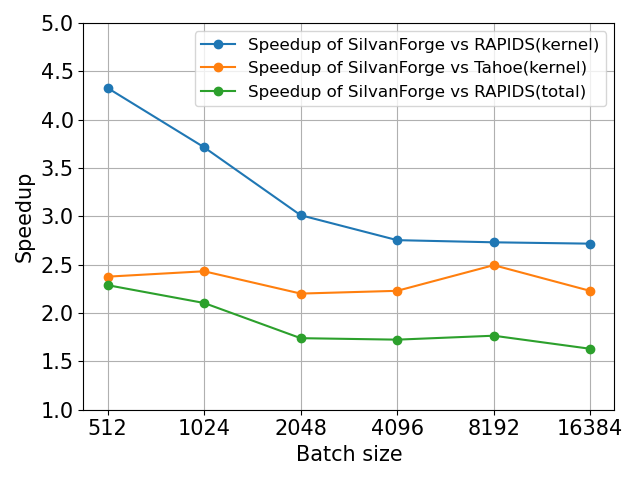
\includegraphics[width=0.75\linewidth]{figures/geomean_speedup_4060_kernel_time_total_time.png}
  \caption{\Treebeard{} vs RAPIDs and Tahoe kernel time and total time speedup on NVIDIA RTX 4060}
  \label{Fig:TBvsRAPIDsTahoe_4060_Speedup}
\end{figure}

% \begin{figure}[htb]
%   \centering
%   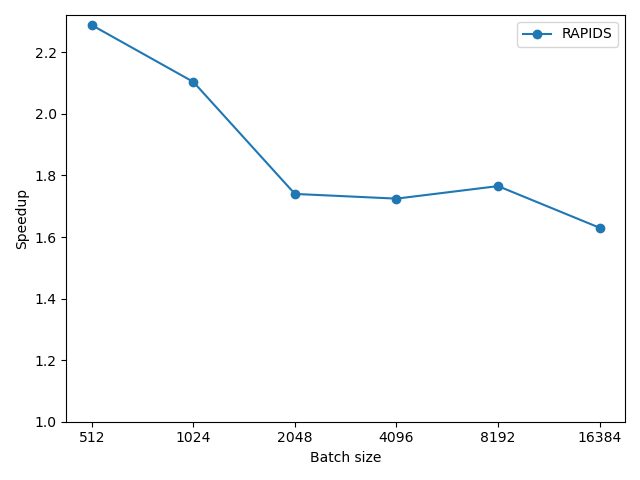
\includegraphics[width=0.75\linewidth]{figures/geomean_speedup_4060_total_time.png}
%   \caption{\Treebeard{} vs RAPIDs Total Time Speedup on NVIDIA RTX 4060.}
%   \label{Fig:TBvsRAPIDs_4060_TotalTimeSpeedup}
% \end{figure}

\begin{figure*}[ht]
  \centering
  \begin{subfigure}[b]{.45\textwidth}
    \subcaptionbox*{}{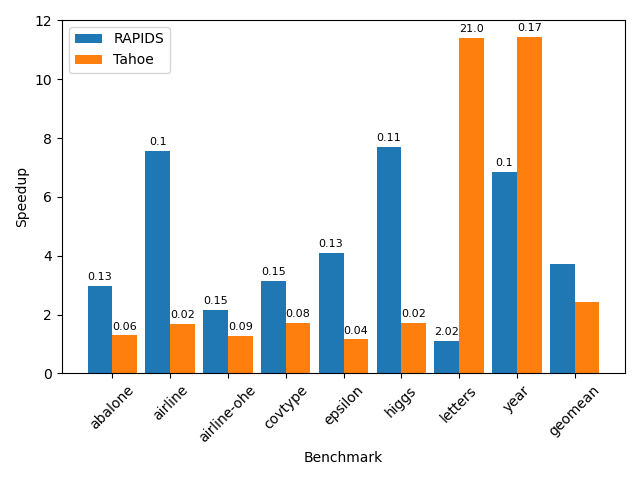
\includegraphics[width=\textwidth]{figures/speedup_bar_graph_1024.png}}
    \caption{Batch size 1024}
  \end{subfigure}
  \begin{subfigure}[b]{.45\textwidth}
    \subcaptionbox*{}{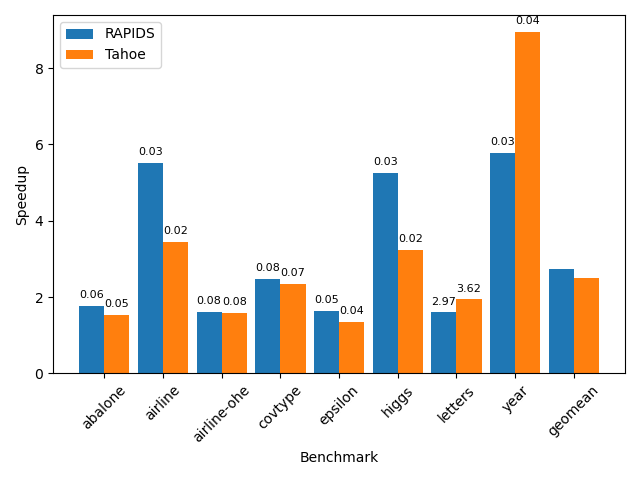
\includegraphics[width=\textwidth]{figures/speedup_bar_graph_8192.png}}
    \caption{Batch size 8192}
  \end{subfigure}
  \hfill
  \caption{\label{Fig:KernelTimeIndividualBenchmarks4060}Kernel time speedup of \Treebeard{} vs RAPIDs on NVIDIA RTX 4060. Numbers on the bars are 
  inference times per sample in $\mu$s for RAPIDs and Tahoe.}
\end{figure*}

\begin{figure}[htb]
  \centering
  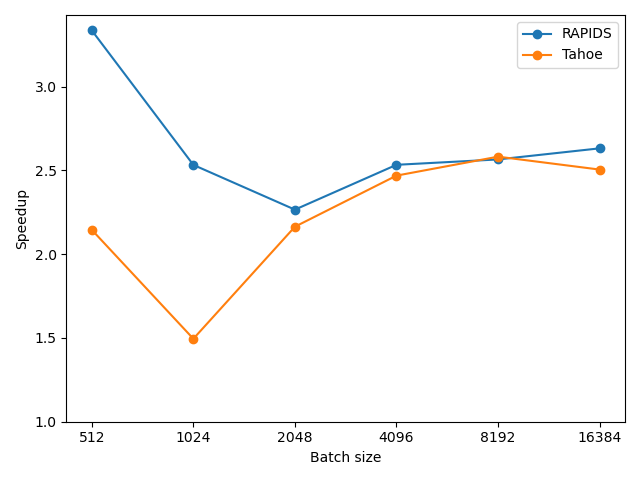
\includegraphics[width=0.75\linewidth]{figures/geomean_speedup_T400_kernel_time.png}
  \caption{\Treebeard{} vs RAPIDs and Tahoe Kernel Time Speedup on NVIDIA T400.}
  \label{Fig:TBvsRAPIDsTahoe_T400_Speedup}
\end{figure}

% \begin{figure*}[ht]
%   \centering
%   \begin{subfigure}[b]{.45\textwidth}
%     \subcaptionbox*{}{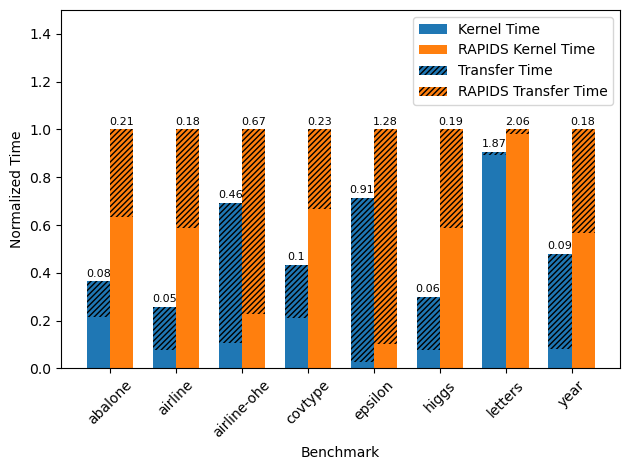
\includegraphics[width=\textwidth]{figures/abs_times_bar_graph_1024.png}}
%     \caption{Batch size 1024.}
%   \end{subfigure}
%   \begin{subfigure}[b]{.45\textwidth}
%     \subcaptionbox*{}{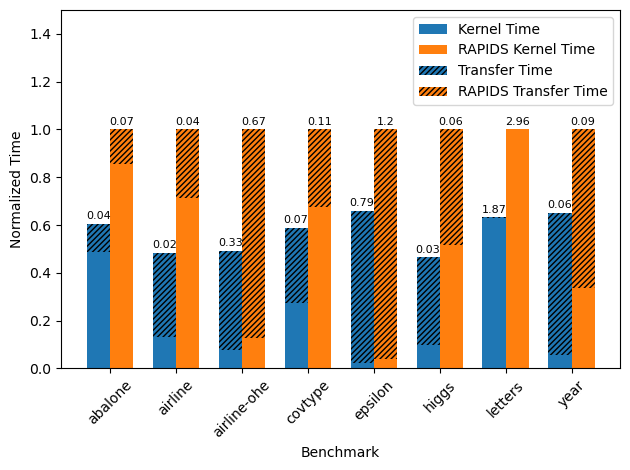
\includegraphics[width=\textwidth]{figures/abs_times_bar_graph_8192.png}}
%     \caption{Batch size 8192.}
%   \end{subfigure}
%   \hfill
%   \caption{\label{Fig:TotalTimeIndividualBenchmarks4060}\Treebeard{} vs RAPIDs total time comparison on NVIDIA RTX 4060. Numbers on the bars are the times 
%   per sample in $\mu$s for \Treebeard{} and RAPIDs. Times for each benchmark are normalized w.r.t the RAPIDs time for that benchmark.}
% \end{figure*}

\begin{figure}[htb]
  \centering
  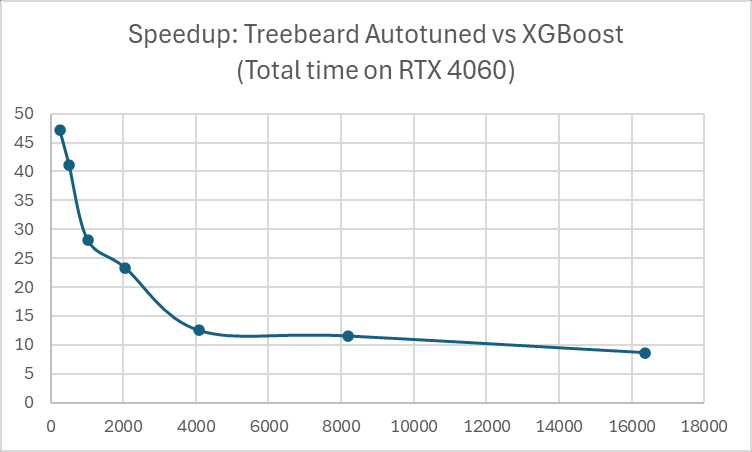
\includegraphics[width=0.75\linewidth]{figures/TBvsXGB_TotalTime.png}
  \caption{\Treebeard{} vs XGBoost Speedup on RTX 4060.}
  \label{Fig:TBvsXGBoost_Speedup}
\end{figure}

\subsection{Autotuning Heuristic}
\begin{figure}[htb]
  \centering
  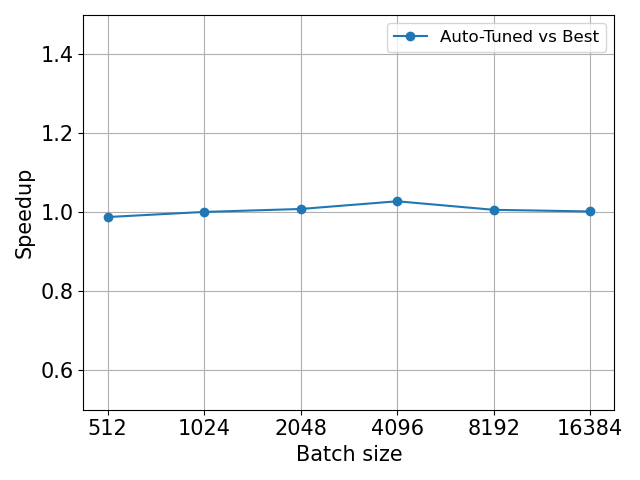
\includegraphics[width=0.75\linewidth]{figures/geomean_speedup_4060_best_vs_at.png}
  \caption{Autotuning heuristics speedup vs best 4060 schedule on NVIDIA RTX 4060}
  \label{Fig:AutotuningSpeedupvs4060Sched}
\end{figure}

\begin{figure}[htb]
  \centering
  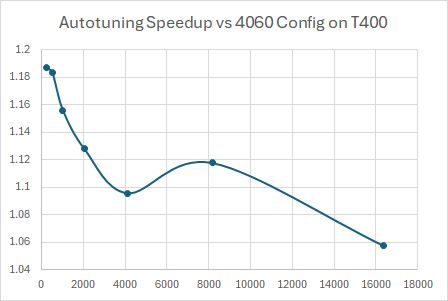
\includegraphics[width=0.75\linewidth]{figures/AutotuningSpeedupvs4060Sched_T400.png}
  \caption{Autotuning heuristics speedup vs best 4060 schedule on T400.}
  \label{Fig:AutotuningSpeedupvs4060Sched_T400}
\end{figure}

\begin{figure}[htb]
  \centering
  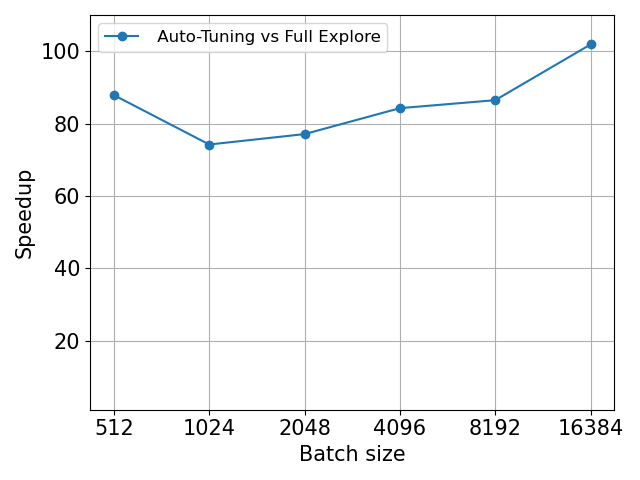
\includegraphics[width=0.75\linewidth]{figures/geomean_speedup_4060_full_exp_vs_at.png}
  \caption{Autotuning heuristic compile time speedup vs full schedule exploration.}
  \label{Fig:HeuristicVsFullExplore_Speedup}
\end{figure}

\begin{itemize}
  \item We compare the schedule found by the schedule exploration heuristic on the RTX 4060 with the best schedule found by
  extensive exploration. Figure \ref{Fig:HeuristicVsFullExplore_Speedup} shows that the heuristic is able to find schedules that are
  very close to the best schedule found by exhaustive exploration.
  \item The speedup of the heuristic schedule vs the best 4060 schedule is shown in Figure \ref{Fig:AutotuningSpeedupvs4060Sched}.
  Geomean speedup range from 1.1$\times$ to 1.2$\times$.
  \item 
\end{itemize}

\subsection{AMD GPU}
\begin{figure}[htb]
  \centering
  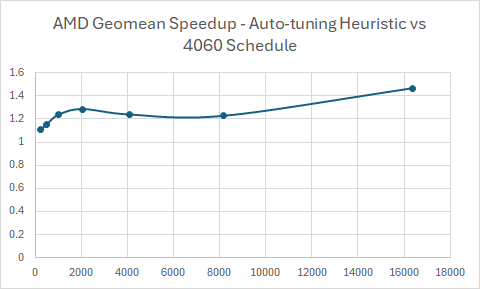
\includegraphics[width=0.75\linewidth]{figures/AMD_MI210_ATHeuristicVs4060Sched_speedup.png}
  \caption{Autotuning heuristics speedup vs best 4060 schedule on MI210.}
  \label{Fig:AMD_MI210_ATHeuristicVs4060Sched_speedup}
\end{figure}

\subsection{CPU Improvements}
\begin{itemize}
  \item The ability of \Treebeard{} to parallelize across both trees and rows has a significant impact on CPU performance.
  \item We run experiments on the Intel Core i9-11900K processor to evaluate the impact of parallelizing across trees with small batch sizes. 
  \item At batch size 32, we find that the average speedup over all 8 models is 2.2$\times$ with a max speedup of 5$\times$.
  \item At batch size 64, we find that the average speedup over all 8 models is 1.1$\times$ with a max speedup of 2$\times$. 
  However, we find that 2 of the 8 models show slowdowns in this case. Again, this highlights the need for schedule exploration on CPUs.
  \item For small batch sizes, parallelizing across rows does not work great since there is limited reuse of trees in L1 cache.
  Also, the amount of work per thread is very small leading to high overheads. 
  \item Parallelizing across trees is more effective since there is more reuse in L1 cache and the amount of work per thread is higher.  
\end{itemize}